\section{Prozessmodelle}
	
\begin{itemize}
\item \textbf{Programmieren durch Probieren} (Trial \& Error)
\begin{itemize}
\item \textbf{Programm erzeugen und danach alles weitere} planen, testen, warten,..
				
\begin{center}
\begin{tabular}{c|c}
\color{green}{\textbf{+}} & \color{red}{\textbf{-}} \\
\hline
- Schnell & - Schlecht strukturiert \\
- Ohne nutzlosen Zusatzaufwand & - Keine Dokumentation
\end{tabular}
\end{center}
\end{itemize}
\item \textbf{Wasserfallmodell}
\begin{itemize}
\item \textbf{Dokumentgetriebenes Modell}
\item \textbf{Jede Aktivität in fester Reihenfolge} und anschließendem Dokument
				
\begin{center}
\begin{tabular}{c|c}
\color{green}{\textbf{+}} & \color{red}{\textbf{-}} \\
\hline
- Einfach & - Entwurf, Implementierung und Testen von nutzlosem Code \\
- Verständlich & - Keine Rückkopplung
\end{tabular}
\end{center}
\end{itemize}
\item \textbf{V-Modell 97} (Vorgehensmodell)
\begin{itemize}
\item Jede Aktivität hat \textbf{eigenen Prüfungsschritt}
\end{itemize}
\end{itemize}
		
\begin{center}
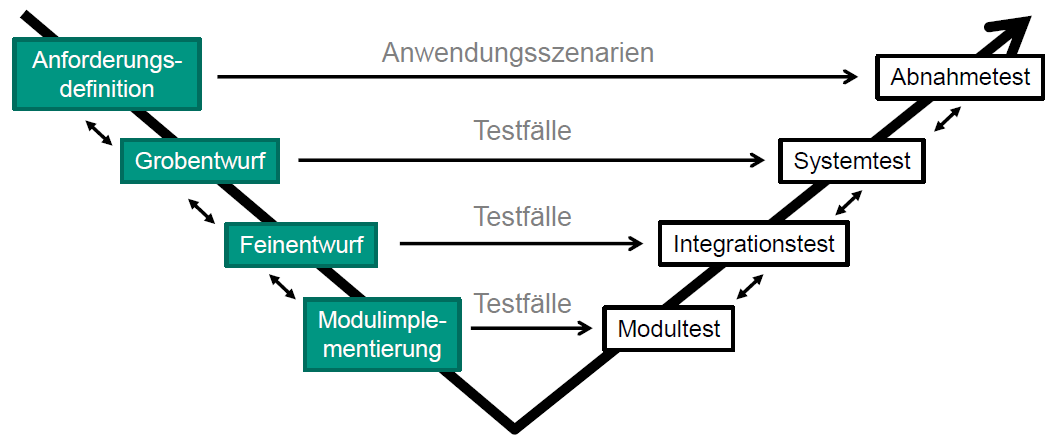
\includegraphics[width=0.9\textwidth]{../images/vmodell97.png}
\end{center}
				
\newpage
\begin{itemize}
\item \textbf{V-Modell XT}
\begin{itemize}
\item Entwicklungsstandard für IT-Systeme der \textbf{öffentlichen Hand}
\item \textbf{Aktivitäten, Produkte und Verantwortlichkeit} werden festgelegt, jedoch \underline{keine} Reihenfolge
\item Aufteilung in \textbf{vier Submodelle} mit zusätzlichen \textbf{Vorgehensbausteinen}:
\begin{itemize}
\item \textbf{Projektmanagement}
\item \textbf{Qualitätssicherung}
\item \textbf{Konfigurationsmanagement}
\item \textbf{Systemerstellung}
\end{itemize}
\end{itemize}
\item \textbf{Prototypmodell}
\begin{itemize}
\item Geeignet für Systeme, für die keine vollständige Spezifikation \textbf{ohne explorative Entwicklung/Experimentation} erstellt werden kann
\item Prototyp wird \textbf{WEGGEWORFEN!}
\end{itemize}
\item \textbf{Iteratives Modell}
\begin{itemize}
\item \textbf{Teile der Funktionalität} lassen sich \underline{klar} definieren/realisieren
\begin{itemize}
\item Funktionalität wird \textbf{Schritt für Schritt} hinzugefügt
\end{itemize}
\end{itemize}
\item \textbf{Synchronisiere und Stabilisiere}
\begin{itemize}
\item Idee:
\end{itemize}
			
\begin{center}
\begin{tabular}{c}
Programmierer in \textbf{kleinen Teams} \\
$\Downarrow$ \\
Regelmäßig \textbf{synchronisieren} (nächtlich) \\
$\Downarrow$ \\
Regelmäßig \textbf{stabilisieren} (3-Monate) \\
\end{tabular}
\end{center}
			
\newpage
\begin{itemize}			
\item \textbf{Phasen:}
\begin{itemize}
\item \textbf{Planungsphase} (3-12 Monate)
\begin{itemize}
\item Wunschbild, Spezifikation, Zeitplan und Teamstruktur
\end{itemize}
\item \textbf{Entwicklungsphase} (6-12 Monate)
\begin{itemize}
\item Manager koordinieren, Entwickler entwerfen und Tester testen parallel
\end{itemize}
\item \textbf{Stabilisierungsphase} (3-8 Monate)
\begin{itemize}
\item Manager koordinieren Beta-Tester und sammeln Rückmeldungen
\item Entwickler stabilisieren Code
\item Tester isolieren Fehler
\end{itemize}
\end{itemize}
\end{itemize}
\end{itemize}
					
\begin{center}
\resizebox{\textwidth}{!}{
\begin{tabular}{c|c}
\color{green}{\textbf{+}} & \color{red}{\textbf{-}} \\
\hline
- Effektiv durch kurze Produktzyklen & - Ungeeignet für manche Art von Softwareproblemen \\
- Fortschritt ohne vollständige Spezifikation & - Mangelnde Fehlertoleranz oder Echtzeitfähigkeit
\end{tabular}}
\end{center}
	
\subsection{Agile Prozessmodelle}
	
\begin{itemize}
\item Idee:
\begin{itemize}
\item \textbf{Minimum} an Vorausplanung
\item Planung erfolgt \textbf{inkrementell}
\item \textbf{Schnelle Reaktion} auf Änderung
\end{itemize}

\newpage
\item Vertreter:
\begin{itemize}
\item \textbf{Extreme Programming} (XP)
\item \textbf{Scrum!}
\item Crystal
\item Adaptive Software Development
\item Feature-Driven Development
\item Software Expedition
\end{itemize}
\end{itemize}
			
\subsubsection{Extreme Programming}
	
\begin{itemize}
\item \textbf{Paarprogrammierung}
\begin{itemize}
\item \underline{Zwei} Entwickler an \underline{einer} Maus/Tastatur
\item Geeignet für:
\begin{itemize}
\item \textbf{Vage und schnell ändernde} Anforderungen
\item \textbf{Kleines} Entwicklerteam
\item \textbf{Wenig} Verwaltungsaufwand
\end{itemize}
\end{itemize}
\end{itemize}
			
\begin{center}
\resizebox{\textwidth}{!}{
\begin{tabular}{c|c}
\color{green}{\textbf{+}} & \color{red}{\textbf{-}} \\
\hline
- Bessere Qualität des Quellcodes & - Doppelte Kosten \\
- Gut für unerfahrene Entwickler & - Vorteil gegenüber einzelner Programmierung \\ 
& mit Inspektionen nicht nachweisbar
\end{tabular}}
\end{center}
		
\newpage
\subsubsection{Scrum}
			
\begin{itemize}
\item Vorgehensmodell: \textbf{Agiles Projektmanagement}
\item \textbf{Artefakte:}
\begin{itemize}
\item \textbf{Anforderungsliste} (Product backlog)
\begin{itemize}
\item \underline{Produktanforderungen} und Liste aller \underline{Projektarbeiten}
\item Anforderungen vor jedem Sprint \underline{priorisiert}
\end{itemize}
\item \textbf{Aufgabenliste} (Sprint backlog)
\begin{itemize}
\item Alle Aufgaben mit Beschreibungen für \underline{aktuellen Sprint}
\end{itemize}
\item \textbf{Hindernisliste} (Impediment backlog)
\begin{itemize}
\item Alle \underline{Hindernisse des Projekts}, die Scrum-Master mit Team bespricht
\end{itemize}
\end{itemize}
\item \textbf{Rollen:}
\begin{itemize}
\item \textbf{Auftraggeber} (Product owner)
\begin{itemize}
\item Legt \underline{Anforderungen/Auslieferungstermin} fest
\item Stellt \underline{Budget}
\item \underline{Priorisiert} Anforderungen für Sprint
\end{itemize}
\item \textbf{Scrum-Master}
\begin{itemize}
\item Sicherstellung der \underline{Scrumwerte und -techniken}
\item Sorgt sich um \underline{vollständiges, funktionsfähiges und produktives Team}
\item \underline{Beseitigt Hindernisse} und kommuniziert zwischen den Rollen
\end{itemize}
\item \textbf{Entwicklungsteam}
\begin{itemize}
\item Personen \underline{unterschiedlicher Fachrichtungen}
\end{itemize}
\end{itemize}

\newpage
\item \textbf{Treffen:}
\begin{itemize}
\item \textbf{Sprintplanung}
\begin{itemize}
\item Entwicklungsteam wählt \underline{machbare Anforderungen} aus, die im Sprint geschafft werden kann und erstellt mit Scrum-Master eine Aufgabenliste
\end{itemize}
\item \textbf{Tägliches Scrumtreffen} (Daily Scrum)
\begin{itemize}
\item \dq Was hast du gestern getan?\dq
\item \dq Was wirst du heute tun?\dq
\item \dq Welche Hindernisse gibt es?\dq
\end{itemize}
\item \textbf{Reviewtreffen} (Sprintende)
\begin{itemize}
\item Vorstellen der \underline{Sprintergebnisse}
\item \underline{Keine} Folien!
\end{itemize}
\item \textbf{Retrospektive}
\begin{itemize}
\item \underline{Analyse vom letzten Sprint} mit dem Entwicklungsteam, Scrum-Master, Auftraggeber und eventuell dem Endkunden
\end{itemize}
\end{itemize}
\end{itemize}